% Options for packages loaded elsewhere
\PassOptionsToPackage{unicode}{hyperref}
\PassOptionsToPackage{hyphens}{url}
%
\documentclass[
]{article}
\usepackage{lmodern}
\usepackage{amssymb,amsmath}
\usepackage{ifxetex,ifluatex}
\ifnum 0\ifxetex 1\fi\ifluatex 1\fi=0 % if pdftex
  \usepackage[T1]{fontenc}
  \usepackage[utf8]{inputenc}
  \usepackage{textcomp} % provide euro and other symbols
\else % if luatex or xetex
  \usepackage{unicode-math}
  \defaultfontfeatures{Scale=MatchLowercase}
  \defaultfontfeatures[\rmfamily]{Ligatures=TeX,Scale=1}
\fi
% Use upquote if available, for straight quotes in verbatim environments
\IfFileExists{upquote.sty}{\usepackage{upquote}}{}
\IfFileExists{microtype.sty}{% use microtype if available
  \usepackage[]{microtype}
  \UseMicrotypeSet[protrusion]{basicmath} % disable protrusion for tt fonts
}{}
\makeatletter
\@ifundefined{KOMAClassName}{% if non-KOMA class
  \IfFileExists{parskip.sty}{%
    \usepackage{parskip}
  }{% else
    \setlength{\parindent}{0pt}
    \setlength{\parskip}{6pt plus 2pt minus 1pt}}
}{% if KOMA class
  \KOMAoptions{parskip=half}}
\makeatother
\usepackage{xcolor}
\IfFileExists{xurl.sty}{\usepackage{xurl}}{} % add URL line breaks if available
\IfFileExists{bookmark.sty}{\usepackage{bookmark}}{\usepackage{hyperref}}
\hypersetup{
  pdftitle={Progress report: Detecting interaction with unknown environmental covariate},
  pdfauthor={Ziang Zhang},
  hidelinks,
  pdfcreator={LaTeX via pandoc}}
\urlstyle{same} % disable monospaced font for URLs
\usepackage[margin=1in]{geometry}
\usepackage{color}
\usepackage{fancyvrb}
\newcommand{\VerbBar}{|}
\newcommand{\VERB}{\Verb[commandchars=\\\{\}]}
\DefineVerbatimEnvironment{Highlighting}{Verbatim}{commandchars=\\\{\}}
% Add ',fontsize=\small' for more characters per line
\usepackage{framed}
\definecolor{shadecolor}{RGB}{248,248,248}
\newenvironment{Shaded}{\begin{snugshade}}{\end{snugshade}}
\newcommand{\AlertTok}[1]{\textcolor[rgb]{0.94,0.16,0.16}{#1}}
\newcommand{\AnnotationTok}[1]{\textcolor[rgb]{0.56,0.35,0.01}{\textbf{\textit{#1}}}}
\newcommand{\AttributeTok}[1]{\textcolor[rgb]{0.77,0.63,0.00}{#1}}
\newcommand{\BaseNTok}[1]{\textcolor[rgb]{0.00,0.00,0.81}{#1}}
\newcommand{\BuiltInTok}[1]{#1}
\newcommand{\CharTok}[1]{\textcolor[rgb]{0.31,0.60,0.02}{#1}}
\newcommand{\CommentTok}[1]{\textcolor[rgb]{0.56,0.35,0.01}{\textit{#1}}}
\newcommand{\CommentVarTok}[1]{\textcolor[rgb]{0.56,0.35,0.01}{\textbf{\textit{#1}}}}
\newcommand{\ConstantTok}[1]{\textcolor[rgb]{0.00,0.00,0.00}{#1}}
\newcommand{\ControlFlowTok}[1]{\textcolor[rgb]{0.13,0.29,0.53}{\textbf{#1}}}
\newcommand{\DataTypeTok}[1]{\textcolor[rgb]{0.13,0.29,0.53}{#1}}
\newcommand{\DecValTok}[1]{\textcolor[rgb]{0.00,0.00,0.81}{#1}}
\newcommand{\DocumentationTok}[1]{\textcolor[rgb]{0.56,0.35,0.01}{\textbf{\textit{#1}}}}
\newcommand{\ErrorTok}[1]{\textcolor[rgb]{0.64,0.00,0.00}{\textbf{#1}}}
\newcommand{\ExtensionTok}[1]{#1}
\newcommand{\FloatTok}[1]{\textcolor[rgb]{0.00,0.00,0.81}{#1}}
\newcommand{\FunctionTok}[1]{\textcolor[rgb]{0.00,0.00,0.00}{#1}}
\newcommand{\ImportTok}[1]{#1}
\newcommand{\InformationTok}[1]{\textcolor[rgb]{0.56,0.35,0.01}{\textbf{\textit{#1}}}}
\newcommand{\KeywordTok}[1]{\textcolor[rgb]{0.13,0.29,0.53}{\textbf{#1}}}
\newcommand{\NormalTok}[1]{#1}
\newcommand{\OperatorTok}[1]{\textcolor[rgb]{0.81,0.36,0.00}{\textbf{#1}}}
\newcommand{\OtherTok}[1]{\textcolor[rgb]{0.56,0.35,0.01}{#1}}
\newcommand{\PreprocessorTok}[1]{\textcolor[rgb]{0.56,0.35,0.01}{\textit{#1}}}
\newcommand{\RegionMarkerTok}[1]{#1}
\newcommand{\SpecialCharTok}[1]{\textcolor[rgb]{0.00,0.00,0.00}{#1}}
\newcommand{\SpecialStringTok}[1]{\textcolor[rgb]{0.31,0.60,0.02}{#1}}
\newcommand{\StringTok}[1]{\textcolor[rgb]{0.31,0.60,0.02}{#1}}
\newcommand{\VariableTok}[1]{\textcolor[rgb]{0.00,0.00,0.00}{#1}}
\newcommand{\VerbatimStringTok}[1]{\textcolor[rgb]{0.31,0.60,0.02}{#1}}
\newcommand{\WarningTok}[1]{\textcolor[rgb]{0.56,0.35,0.01}{\textbf{\textit{#1}}}}
\usepackage{graphicx,grffile}
\makeatletter
\def\maxwidth{\ifdim\Gin@nat@width>\linewidth\linewidth\else\Gin@nat@width\fi}
\def\maxheight{\ifdim\Gin@nat@height>\textheight\textheight\else\Gin@nat@height\fi}
\makeatother
% Scale images if necessary, so that they will not overflow the page
% margins by default, and it is still possible to overwrite the defaults
% using explicit options in \includegraphics[width, height, ...]{}
\setkeys{Gin}{width=\maxwidth,height=\maxheight,keepaspectratio}
% Set default figure placement to htbp
\makeatletter
\def\fps@figure{htbp}
\makeatother
\setlength{\emergencystretch}{3em} % prevent overfull lines
\providecommand{\tightlist}{%
  \setlength{\itemsep}{0pt}\setlength{\parskip}{0pt}}
\setcounter{secnumdepth}{5}

\title{Progress report: Detecting interaction with unknown environmental
covariate}
\author{Ziang Zhang}
\date{15/10/2020}

\begin{document}
\maketitle

\hypertarget{summary-of-current-progress}{%
\section{Summary of current
progress:}\label{summary-of-current-progress}}

\hypertarget{latent-model-for-binary-data}{%
\subsection{Latent Model for binary
data}\label{latent-model-for-binary-data}}

For binary response variable, it is often assumed that the reponse
variable \(y_i\) conditioning on the regressors \(G_i,Z_i\) come from a
latent model such that: \begin{equation}\label{eqn:latentformulation}
\begin{aligned}
Y_i^* &= \beta_0 + \beta_G G_i + \beta_Z Z_i + \epsilon_i \\
Y_i &= I\{Y_i^*>0\} \\
\end{aligned}
\end{equation}

The unobserved latent variable \(Y_i^*\) determines whether the observed
response variable \(Y_i\) is 0 or 1. The error term \(\epsilon_i\) in
\(Y_i^*\) needs to have a completely known distribution, which can be
\(\text{N}(0,1)\) for the model to become a probit model, or a logistic
distribution with mean 0 and variance 3.28 for the model to become a
logistic regression model.

Here the regressor \(G_i\) represents the allele of interest, and the
regressor \(Z_i\) is any regressor that can be non-genetic.

\hypertarget{method-1-detection-from-linearity}{%
\subsection{Method 1: Detection from
linearity}\label{method-1-detection-from-linearity}}

\hypertarget{when-the-true-model-does-not-contain-interaction-with-environmental-factor}{%
\subsubsection{When the true model does not contain interaction with
environmental
factor}\label{when-the-true-model-does-not-contain-interaction-with-environmental-factor}}

First, consider that the true underlying model for the response variable
\(Y_i\) is a probit model without interaction effect, i.e:
\begin{equation}\label{eqn:probitModel}
\begin{aligned}
Y_i^* &= \beta_0 + \beta_G G_i + \beta_Z Z_i + \epsilon_i \\
Y_i &= I\{Y_i^*>0\} \\
\epsilon_i &\sim \text{N}(0,1)
\end{aligned}
\end{equation}

Therefore, it can be shown that:
\begin{equation}\label{eqn:probitModelLinearity}
\begin{aligned}
\text{P}(Y_i = 1| G_i, Z_i) &= \text{P}(\epsilon_i > -(\beta_0 +\beta_G G_i + \beta_Z Z_i)) \\
&= 1 - \Phi(-(\beta_0 + \beta_G G_i + \beta_Z Z_i)) \\
&= \Phi(\beta_0 + \beta_G G_i + \beta_Z Z_i)
\end{aligned}
\end{equation} Where \(\Phi(.)\) denote the CDF function of standard
normal distribution. Therefore,
\(\Phi^{-1}\bigg(\text{P}(Y_i = 1|G_i,Z_i)\bigg)\) shoud be a linear
function of both \(G_i\) and \(Z_i\).

\hypertarget{when-the-true-model-does-contain-gene-environment-interaction}{%
\subsubsection{When the true model does contain gene-environment
interaction}\label{when-the-true-model-does-contain-gene-environment-interaction}}

Assume for simplicity that \(E_i\) the environmental variable has a
normal distribution with mean \(\mu_E\) and variance \(\sigma_E^2\), and
suppose that the true underlying model is:
\begin{equation}\label{eqn:probitModelWithInteraction}
\begin{aligned}
Y_i^* &= \beta_0 + \beta_G G_i + \beta_Z Z_i + \beta_{G\times E} G_i \times E_i + \epsilon_i \\
Y_i &= I\{Y_i^*>0\} \\
\epsilon_i &\sim \text{N}(0,1)
\end{aligned}
\end{equation}

Furthermore, we can compute that:
\begin{equation}\label{eqn:probitModelWithInteraction_MeanVar}
\begin{aligned}
\text{E}(Y_i^*|G_i,Z_i) &= \beta_0 + (\beta_G + \beta_{G\times E} \mu_E)G_i + \beta_Z Z_i \\
\text{Var}(Y_i^*|G_i,Z_i) &= (\beta_{G\times E} G_i)^2 \sigma_E^2 + 1 \\
Y_i^*|G_i, Z_i &\sim \text{N}\bigg(\beta_0 + (\beta_G + \beta_{G\times E} \mu_E)G_i + \beta_Z Z_i,  \big(\beta_{G\times E} G_i\big)^2 \sigma_E^2 + 1\bigg)
\end{aligned}
\end{equation}

That implies that the probability we get a case for different levels of
\(G_i\) and \(Z_i\) will be:
\begin{equation}\label{eqn:probitModelWithInteraction_Prob} 
\begin{aligned} 
\text{P}(Y = 1 | G_i, Z_i) &= \text{P}(Y^* > 0| G_i, Z_i) \\ 
                           &= \text{P}(\frac{Y^*  - \text{E}(Y^* |G_i,Z_i)}{\sqrt{\text{Var}(Y^* |G_i,Z_i)}} > \frac{-\text{E}(Y^* |G_i,Z_i)}{\sqrt{\text{Var}(Y^* |G_i,Z_i)}}) \\
                           &= \Phi \bigg( \frac{\text{E}(Y^* |G_i,Z_i)}{\sqrt{\text{Var}(Y^* |G_i,Z_i)}} \bigg)
\end{aligned}
\end{equation}

Therefore, applying the inverse CDF on both sides, we get
\[\Phi^{-1} \bigg(\text{P}(Y = 1 | G, Z) \bigg) = \frac{\beta_0+(\beta_G + \beta_{G\times E} \mu_E)G_i + \beta_Z Z}{\sqrt{(\beta_{G\times E}^2 G_i^2 \sigma_E^2 + 1)}} \]

This is not a linear function of \(G_i\), but is a linear function of
\(Z_i\).

\begin{enumerate}
\item If the true underlying model also contains another regressor $W$ but $W$ is uncorrelated with $G$ for example. Then eventhough ignoring that regressor breaks the structural assumption of probit model, so that the fitted model without $W$ is no longer a probit model (since now $\epsilon$ does not follow standard normal), but $\Phi^{-1}(\text{P}(Y_i = 1|G_i,Z_i))$ will still be a linear function of $G_i$. So detecting based on the linearity of $\Phi^{-1}\text{P}$ will not be affected by omitted exogenous regressors.
\item Since $P(Y_i = 1|G_i,Z_i)$ is actually unknown in practice, we can estimate it using the sample proportion $\hat{P}(Y = 1|G = g,Z = z) = \frac{\sum_{i=1}^{n} \text{I}\{y_i =1,G_{i} = g, Z_{i} = z\}}{\sum_{i=1}^{n}  \text{I}\{G_{i} = g, Z_{i} = z\}}$. We shouldn't use the fitted model to estimate them since our fitted model may be wrong.
\item The reason we used probit model instead of logistic model here is that assuming $E$ follows normal distribution, $Y^*|G,Z$ will still be normal if we omit the interaction term, since linear combination of normal is normal. But assuming $E$ follows logistic distribution does not imply that $Y^*|G,Z$ will be logistically distributed as logistic distribution is not closed under linear combination. However, based on the literature, it seems like probit model and logistic model have really closed results in real applications.
\end{enumerate}

\hypertarget{test-statistic-of-this-method}{%
\subsubsection{Test Statistic of this
method:}\label{test-statistic-of-this-method}}

This method relies on the checking of linearity of \(\Phi^{-1}(P)\), so
the test statistics will also be focusing on the detection of linearity.
Depending on the type of data available, there will be several slightly
different test statistics for different cases.

\hypertarget{case-1-when-g-is-the-only-regressor-in-the-model}{%
\paragraph{Case 1: When G is the only regressor in the
model}\label{case-1-when-g-is-the-only-regressor-in-the-model}}

If the two competing models are: \begin{equation}
\begin{aligned}
1. Y_i ^{*} = \beta_0 + \beta_G G_i + \beta_E E_i + \epsilon_i \\
2. Y_i ^{*} = \beta_0 + \beta_G G_i + \beta_E E_i + \beta_{G\times E}G_i \times E_i + \epsilon_i \\
\end{aligned}
\end{equation}

Let \(p_i = P(Y = 1|G=i)\), which can be approximated by the sample
proportion \(\hat{p_i}\). We know that
\[\Phi^{-1}(\hat{p_i}) \sim N\bigg(\Phi^{-1}(p_i), \frac{1}{\phi(\Phi^{-1}(p_i))^2} \frac{p_i(1-p_i)}{n_i}\bigg)\]
Here \(n_i\) denotes the number of \(G = i\) in our dataset. Let
\(v_i = \frac{1}{\phi(\Phi^{-1}(\hat{p_i}))^2} \frac{\hat{p_i}(1-\hat{p_i})}{n_i}\)
denote the estimate of \(Var(\Phi^{-1}(\hat{p_i}))\).

Let
\(S = \Phi^{-1}(\hat{p_2}) - 2\Phi^{-1}(\hat{p_1}) + \Phi^{-1}(\hat{p_0})\),
and \(T = \frac{S^2}{v_o+4v_1+v_2}\) be our test statistic. If 1 is the
true model, then \(T \sim X^2_{1}\).

\hypertarget{case-2-when-both-g-and-z-are-in-the-regression-where-z-is-discrete}{%
\paragraph{Case 2: When both G and Z are in the regression, where Z is
discrete:}\label{case-2-when-both-g-and-z-are-in-the-regression-where-z-is-discrete}}

If the two competing models are: \begin{equation}
\begin{aligned}
1. Y_i ^{*} = \beta_0 + \beta_G G_i + \beta_Z Z_i + \beta_E E_i + \epsilon_i \\
2. Y_i ^{*} = \beta_0 + \beta_G G_i + \beta_Z Z_i + \beta_E E_i + \beta_{G\times E}G_i \times E_i + \epsilon_i \\
\end{aligned}
\end{equation}

Let \(\hat{p_{ij}}\) denote the sample proportion of cases in the group
with \(G = i\) and \(Z = j\), then we know that \(\hat{p_{ij}}\) will be
independent across different i and j. Also, by CLT:
\[\hat{p_{ij}} \sim N(p_{ij},\frac{p_{ij}(1-p_{ij})}{n_{ij}})\] where
\(n_{ij}\) denote the number of observations in the (i,j) cell.

By delta method: we can obtain the distribution of
\(\Phi^{-1}(\hat{p_{ij}})\) being:
\[\Phi^{-1}(\hat{p_{ij}}) \sim N\bigg(\Phi^{-1}(p_{ij}),\frac{1}{\phi(\Phi^{-1}(p_{ij}))^2}\frac{p_{ij}(1-p_{ij})}{n_{ij}}\bigg)\]
where \(\phi\) denotes the density of a standard normal.

Let \(W_{ij} = \Phi^{-1}(\hat{p_{ij}})\). The variance of \(W_{ij}\) can
be estimated as
\(v_{ij} = \frac{1}{\phi(\Phi^{-1}(\hat{p_{ij}}))^2}\frac{\hat{p_{ij}}(1-\hat{p_{ij}})}{n_{ij}}\),
which is simply plugging \(\hat{p_{ij}}\) for the unknown true
probability \(p_{ij}\). Let
\(S_1 = a_0(W_{10}-W_{00}) + a_1(W_{11}-W_{01}) + a_2(W_{12}-W_{02})\)
and
\(S_2 = a_0(W_{20}-W_{10}) + a_1(W_{21}-W_{11}) + a_2(W_{22}-W_{12})\),
where \(a_i\) is weight given to each difference term, such that
\(\sum_{i=0}^2 a_i =0\). If the frequency of \(G\) or \(Z\) is known.
Then \(a_i = P(Z =i)\) when we are testing for the interaction of \(G\)
with \(E\). So \(S_1\) and \(S_2\) will have a nice interpretation being
estimated expected effect of \(G\).

Under the null hypothesis that \(\beta_{G\times E} =0\) which means no
interaction between \(G\) and \(E\), we know that \(\Phi^{-1}(p_{ij})\)
should be linear in i. That is:
\(W_{(i+1)j} - W_{ij} \sim N(b_i,v_{(i+1)j} + v_{ij})\) for all j =
0,1,2. So:
\[S_1 \sim N\bigg(\sum_{i=0}^{2}a_ib_i,\sum_{i=0}^{2}a_i^2(v_{1i}+v_{0i})\bigg)\]

\[S_2 \sim N\bigg(\sum_{i=0}^{2}a_ib_i,\sum_{i=0}^{2}a_i^2(v_{2i}+v_{1i})\bigg)\]

with the covariance between \(S_1\) and \(S_2\) be denoted as C, which
can be computed as:
\[ C = \text{Cov}(S_1,S_2) = -\sum_{i=0}^{2}v_{1i}a_i^2 \]

That means, if the null hypothesis is true,
\[ T = \frac{(S_1-S_2)^2}{\sigma_{S_1}^2+\sigma_{S_2}^2 -2C} \sim X^2_{df=1}\]
We will reject the null hypothesis when \(T\) has a large value.

\textbf{Question to study:} If \(G\) and \(Z\) are uncorrelated, we can
just ignore the \(Z\) variable and use the test statistic in the first
case. Which way will be better?

\hypertarget{case-3-when-both-g-and-z-are-in-the-regression-where-z-is-continuous}{%
\paragraph{Case 3: When both G and Z are in the regression, where Z is
continuous:}\label{case-3-when-both-g-and-z-are-in-the-regression-where-z-is-continuous}}

Under this case, if \(G\) and \(Z\) are uncorrelated, we can just ignore
the variable \(Z\) in the regression and use the test statistic for case
1.

However if \(G\) and \(Z\) are correlated, simply ignoring \(Z\) and use
the test statistic in case 1 will produce invalid result (If significant
p-value is obtained, it may be due to interaction with \(E\), or due to
correlation with \(Z\)).

To handle the case when \(Z\) is a continuous random variable correlated
with \(G\), we could use a likelihood based method, which involves
fitting two models and compare the likelihood ratio. We are going to
talk about that test statistic in the later section for joint testing of
main effect and interaction effect of \(G\).

\hypertarget{relationship-with-linear-regression}{%
\subsubsection{Relationship with linear
regression:}\label{relationship-with-linear-regression}}

\hypertarget{regression-with-three-points}{%
\paragraph{Regression with three
points}\label{regression-with-three-points}}

The test statistic proposed above can be viewed as the Wald test
statistic of the following regression:
\begin{equation}\label{eqn:asWaldTest}
\begin{aligned}
\Phi^{-1}(\hat{p_{i}}) &= \beta_0 + \beta_1 \text{I}\{G_i = 1\} + \beta_2 \text{I}\{G_i = 2\} + \epsilon_i,\quad \text{for} \quad i = 0,1,2 \\
\text{where} \quad &\epsilon = (\epsilon_0, \epsilon_1, \epsilon_2) \sim \text{N}(0,\Omega) \\
\text{where} \quad &\Omega = \begin{bmatrix} v_0 & 0 & 0 \\ 0 & v_1 & 0 \\ 0 & 0 & v_2 \end{bmatrix}
\end{aligned}
\end{equation}

This is a weighted least square with weight matrix \(\Omega\) capturing
the heterokedasticity. We are interested in testing
\(H_0 : 2\beta_1 - \beta_2 = L\beta = 0\) where \(L = (0,2,-1)\). The
Wald statistics to test it will be:
\[ \frac{(L\hat{\beta})^2}{L(X^T \Omega^{-1}X)^{-1}L^T}\] This turns out
to be exactly the same test statistic we used previously
\(\frac{S^2}{v_o+4v_1+v_2}\).

\hypertarget{two-stage-regression-approach}{%
\paragraph{Two stage regression
approach:}\label{two-stage-regression-approach}}

The above relationship can be generalized using the idea of a two stage
regression. In the first stage, we consider the following generalized
linear regression:
\[ E(Y_i|G_i) = \Phi\bigg(\beta_0+ \beta_1 \text{I}(G_i =1) + \beta_2 \text{I}(G_i =2)\bigg)\]

From this generlized linear regression, we obtained the fitted linear
predictors
\(\hat{\eta_i} = \hat{\beta_0}+\hat{\beta_1}\text{I}(G_i =1) + \hat{\beta_2} \text{I}(G_i =2)\).
Then, we fit the following weighted least square regression in the
second stage:
\[ \hat{\eta_i} = \gamma_0 +\gamma_1  \text{I}(G_i =1) + \gamma_2 \text{I}(G_i =2) +\epsilon_i\]
where
\(\epsilon_i \sim N\bigg(0,\frac{\Phi(\hat{\eta_i})(1-\Phi(\hat{\eta_i}))}{\phi(\hat{\eta_i})^2} \bigg)\).
Define the weight matrix
\(W = \text{diag}\{\frac{\Phi(\hat{\eta_i})(1-\Phi(\hat{\eta_i}))}{\phi(\hat{\eta_i})^2}\}\),
then our previous test statistic is just the test statistic of Wald test
of \(H_0:\gamma_2 = 2\gamma_1\).

The intuition behind how this approach works to detect the interaction
between \(G\) and \(E\) can be thought as following. In the first
regression, we are actually trying to get an estimate of
\(\eta = \frac{\text{E}(Y^*|G)}{\sqrt{\text{Var}(Y^*|G)}}\). Recall from
the first section, if there is interaction between \(G\) and \(E\), then
\(\eta\) will be non-linear in \(G\) due to the fact that
\(\text{Var}(Y^*|G)\) will be non-constant (We cannot directly test on
whether \(Y^*\) has constant variance because it is not estimable).
Therefore, if we observe that \(\hat{\eta}\) is linear in \(G\), which
means \(\gamma_2 = \gamma_1\), then we can be reasonable confident that
there is no interaction present in the model.

We can use the first stage regression to obtain accurate estimate of
\(\eta\) because regardless whether \(\eta\) is linear in G, we know
\(\eta\) can be written as a linear model with \(\text{I}(G_i =1)\) and
\(\text{I}(G_i =2)\). This suggests, if we have another covariate \(Z\)
in the model, we can just do the two stage regressions with all of
\(\text{I}(G_i =j)\) and \(\text{I}(G_i =j)Z_i\) (Then in our null
hypothesis, besides that \(\gamma_2 = 2 \gamma_1\), we can also add
additional constraints that all of \(\text{I}(G_i =j)Z_i\) should have
the same slopes to increase our power).

\hypertarget{joint-testing-of-main-effect-and-interaction-effect-of-g}{%
\subsubsection{Joint Testing of main effect and interaction effect of
G:}\label{joint-testing-of-main-effect-and-interaction-effect-of-g}}

Suppose that we have the following true latent model:
\[ Y_i ^{*} = \beta_0 + \beta_G G_i + \beta_Z Z_i + \beta_E E_i + \beta_{G\times E}G_i \times E_i + \epsilon_i \].
Then like we have derived in the previous section, we know that:
\[Y_i^*|G_i, Z_i \sim \text{N}\bigg(\beta_0 + (\beta_G + \beta_{G\times E} \mu_E)G_i + \beta_Z Z_i,  \big(\beta_{G\times E} G_i\big)^2 \sigma_E^2 + 1\bigg)\]
Assume without loss of generality that \(E\) has been standardized to
\(\text{N}(0,1)\), and define \(\gamma = \beta_{G\times E}^2\), then the
above model can be simplified into:
\[Y_i^*|G_i, Z_i \sim \text{N}\bigg(\beta_0 + \beta_GG_i + \beta_ZZ_i,\ \gamma G^2 + 1\bigg)\]

This model is identifiable, and we can fit it using maximum likelihood
estimation (Actually there is a Rpackage that can fit \(Y^*\) with
variance \(\text{exp}(\gamma G)\), called heteroskedastic probit model
in econometrics. However, for our proposed model, it seems like we do
need to write a Rfunction by ourselves to get the MLE). We can do joint
testing of interaction effect by testing \(H_0: \gamma = 0\), using
likelihood ratio test. Since \(\gamma \geq 0\), we do need to do a
correction for boundary so our LRT test statistic follows
\(X^2_{0}/2 +X^2_{1}/2\) under null hypothesis.

If we want to jointly test
\(H_0: \gamma = 0 \ \text{and} \ \beta_G =0\), we can use a similar LRT
procedure with null distribution being \(X^2_{1}/2 +X^2_{2}/2\).

\hypertarget{method-2-by-modeling-the-interaction-term-as-a-random-slope}{%
\subsection{Method 2: By modeling the interaction term as a random
slope:}\label{method-2-by-modeling-the-interaction-term-as-a-random-slope}}

First, let's rewrite our previous latent variable specification:
\begin{equation}\label{eqn:latentformulationRandomSlope}
\begin{aligned}
Y_i^* &= \beta_0 + \beta_G G_i + \beta_Z Z_i + \beta_{G\times E} G_i \times E_i + \epsilon_i \\
      &= \beta_0 + \beta_G G_i + \beta_Z Z_i + U_i * G_i + \epsilon_i \\
Y_i &= I\{Y_i^*>0\} \\
U_i &= \beta_{G\times E} * E_i
\end{aligned}
\end{equation}

Here \(U_i\) can be thought as a random effect (random slope), being
drawn from distribution \(\text{N}(0,\sigma_u^2)\). Notice that
\(\sigma_u^2 = \beta_{G\times E}^2 \sigma_E^2\). Therefore, testing for
\(\beta_{G\times E} =0\) is equivalent to testing \(\sigma_u^2 = 0\) for
the random effects. In this case, we do not need to restrict our
distribution to the probit model anymore. Since both probit model and
logistic model are flexible enough to incorporate an observations-level
random slopes. (There shouldn't be any identifiability problem with have
too many random slopes(same number as observations), as including an
observations-level random intercepts is a common trick to account for
overdispersion in Poisson regression.)

\hypertarget{test-statistic-for-method-2}{%
\subsubsection{Test statistic for Method
2:}\label{test-statistic-for-method-2}}

In this case, we can use the likelihood Ratio test to test the model
with and without the random slopes, with correction to the boundary.
Therefore, the final test statistic will be
\(-2\Lambda \sim 0.5X^2_1 + 0.5X^2_0\) under null hypothesis.

\textbf{Question to study:} The test statistic for method 2 seems to be
similar to the LRT test statistic used in method 1 for joint testing of
main effects and interaction effects. Are they actually mathematically
the same?

\hypertarget{difference-between-two-potential-methods}{%
\subsection{Difference between two potential
methods}\label{difference-between-two-potential-methods}}

\begin{enumerate}
\item The first method relies on the assumption that the true underlying model is probit model, and the distribution of $E$ is normal. These assumptions shouldn't be too restrictive as it is said in the literature that probit model and logistic model tend to give similar results. However, the second method can be used for both probit model and logistic model. The only assumption in the second method is that $E$ follows a normal distribution.
\item The next step for the first method is to develop a test statistic for testing the linearity. While for the second method, it seems like there are plenty of tools of testing at boudnary to test $\sigma_u = 0$, using likelihood ratio. It seems like in the second method, jointly testing for the main effect and interaction effect 
\item For the simulations of sample size 300000, the first method is very efficent to compute as it basically just computes nine sample proportions and compute their difference. If we can find a good test statistic for this, the hypothesis testing will be efficient to carry out and scale to larger sample. The second method takes a very long time to converge when the interaction is actually present in the model, and lme4 tends to give some warnings about the potential convergence problems if a probit model is fitted and underlying model has the interaction effect. For a larger sample with more regressors, the computational loads will be bigger for the second method.

\end{enumerate}

\hypertarget{simulation-study}{%
\subsection{Simulation study:}\label{simulation-study}}

Here we will implement our previously proposed methods, and see how they
perform to detect the interaction

\hypertarget{method-1}{%
\subsubsection{Method 1:}\label{method-1}}

Take sample size being 3000, and assume that \(G\) has minor allele
frequency 0.2 and \(E\)'s distribution has been standardized. Let's do
four examples with strong interaction effect, medium interaction effect,
small interaction effect and negligible interaction effect:

\begin{Shaded}
\begin{Highlighting}[]
\CommentTok{#### With strong interaction:}
\KeywordTok{set.seed}\NormalTok{(}\DecValTok{123}\NormalTok{)}
\NormalTok{p_val0 <-}\StringTok{ }\KeywordTok{Simulator_One_G}\NormalTok{(}\DataTypeTok{beta0 =} \FloatTok{-1.2}\NormalTok{, }\DataTypeTok{betaG =} \FloatTok{0.8}\NormalTok{, }\DataTypeTok{betaE =} \FloatTok{0.6}\NormalTok{, }\DataTypeTok{betaGE =} \FloatTok{1.5}\NormalTok{, }\DataTypeTok{muE =} \DecValTok{0}\NormalTok{, }\DataTypeTok{sdE =} \DecValTok{1}\NormalTok{, }\DataTypeTok{p1 =} \FloatTok{0.2}\NormalTok{, }\DataTypeTok{size =} \DecValTok{3000}\NormalTok{, }\DataTypeTok{num_trails =} \DecValTok{5000}\NormalTok{)}
\KeywordTok{hist}\NormalTok{(p_val0,}\DataTypeTok{breaks =} \DecValTok{20}\NormalTok{, }\DataTypeTok{freq =}\NormalTok{ F)}
\end{Highlighting}
\end{Shaded}

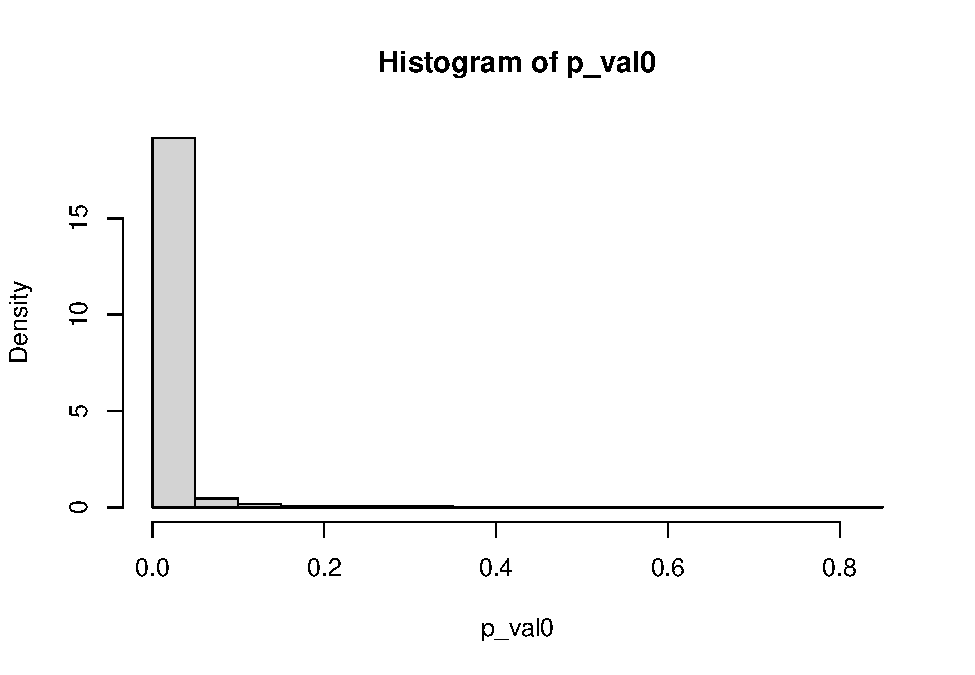
\includegraphics{stats-gene-research-progress-v4_files/figure-latex/unnamed-chunk-1-1.pdf}

\begin{Shaded}
\begin{Highlighting}[]
\CommentTok{#### With medium interaction:}
\KeywordTok{set.seed}\NormalTok{(}\DecValTok{123}\NormalTok{)}
\NormalTok{p_val1 <-}\StringTok{ }\KeywordTok{Simulator_One_G}\NormalTok{(}\DataTypeTok{beta0 =} \FloatTok{-1.2}\NormalTok{, }\DataTypeTok{betaG =} \FloatTok{0.8}\NormalTok{, }\DataTypeTok{betaE =} \FloatTok{0.6}\NormalTok{, }\DataTypeTok{betaGE =} \FloatTok{0.8}\NormalTok{, }\DataTypeTok{muE =} \DecValTok{0}\NormalTok{, }\DataTypeTok{sdE =} \DecValTok{1}\NormalTok{, }\DataTypeTok{p1 =} \FloatTok{0.2}\NormalTok{, }\DataTypeTok{size =} \DecValTok{3000}\NormalTok{, }\DataTypeTok{num_trails =} \DecValTok{5000}\NormalTok{)}
\KeywordTok{hist}\NormalTok{(p_val1,}\DataTypeTok{breaks =} \DecValTok{20}\NormalTok{, }\DataTypeTok{freq =}\NormalTok{ F)}
\end{Highlighting}
\end{Shaded}

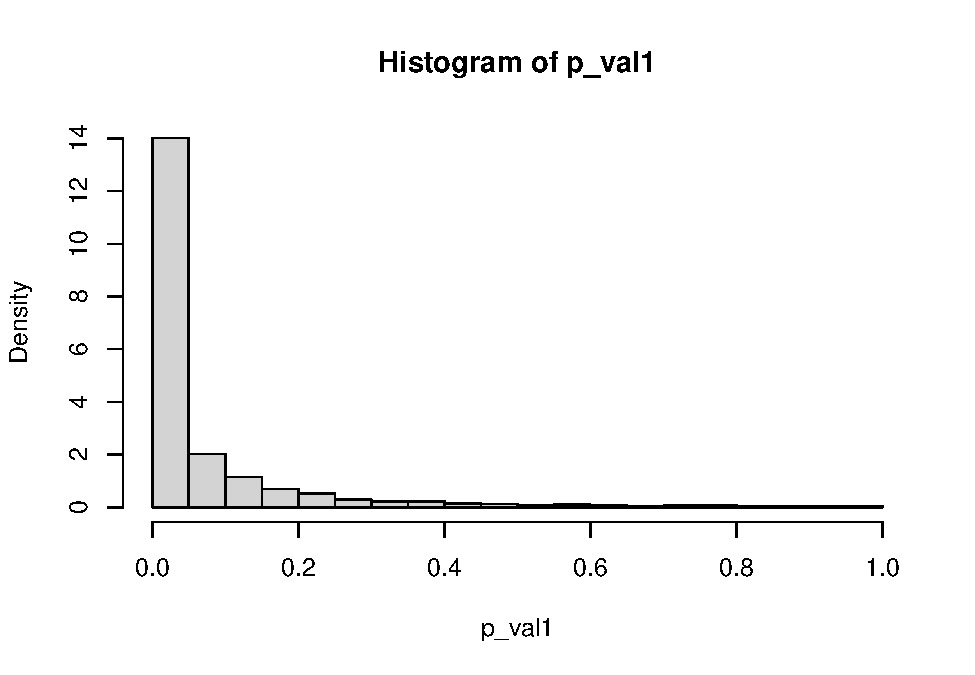
\includegraphics{stats-gene-research-progress-v4_files/figure-latex/unnamed-chunk-1-2.pdf}

\begin{Shaded}
\begin{Highlighting}[]
\CommentTok{#### With small interaction:}
\KeywordTok{set.seed}\NormalTok{(}\DecValTok{123}\NormalTok{)}
\NormalTok{p_val2 <-}\StringTok{ }\KeywordTok{Simulator_One_G}\NormalTok{(}\DataTypeTok{beta0 =} \FloatTok{-1.2}\NormalTok{, }\DataTypeTok{betaG =} \FloatTok{0.8}\NormalTok{, }\DataTypeTok{betaE =} \FloatTok{0.6}\NormalTok{, }\DataTypeTok{betaGE =} \FloatTok{0.3}\NormalTok{, }\DataTypeTok{muE =} \DecValTok{0}\NormalTok{, }\DataTypeTok{sdE =} \DecValTok{1}\NormalTok{, }\DataTypeTok{p1 =} \FloatTok{0.2}\NormalTok{, }\DataTypeTok{size =} \DecValTok{3000}\NormalTok{, }\DataTypeTok{num_trails =} \DecValTok{5000}\NormalTok{)}
\KeywordTok{hist}\NormalTok{(p_val2,}\DataTypeTok{breaks =} \DecValTok{20}\NormalTok{, }\DataTypeTok{freq =}\NormalTok{ F)}
\end{Highlighting}
\end{Shaded}

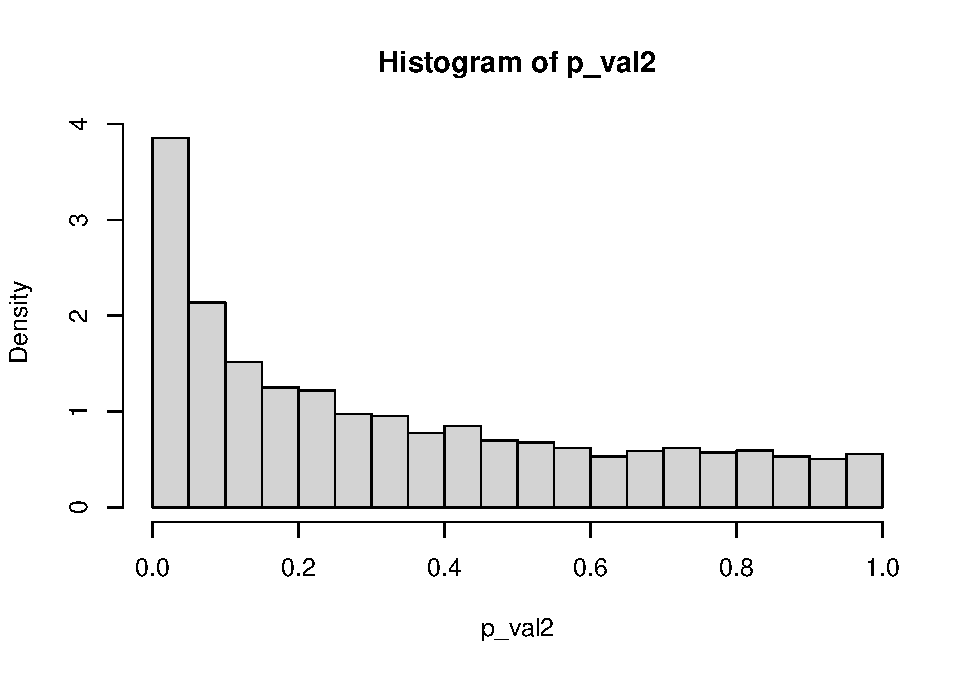
\includegraphics{stats-gene-research-progress-v4_files/figure-latex/unnamed-chunk-1-3.pdf}

\begin{Shaded}
\begin{Highlighting}[]
\CommentTok{#### With negligible interaction:}
\KeywordTok{set.seed}\NormalTok{(}\DecValTok{123}\NormalTok{)}
\NormalTok{p_val3 <-}\StringTok{ }\KeywordTok{Simulator_One_G}\NormalTok{(}\DataTypeTok{beta0 =} \FloatTok{-1.2}\NormalTok{, }\DataTypeTok{betaG =} \FloatTok{0.8}\NormalTok{, }\DataTypeTok{betaE =} \FloatTok{0.6}\NormalTok{, }\DataTypeTok{betaGE =} \FloatTok{0.03}\NormalTok{, }\DataTypeTok{muE =} \DecValTok{0}\NormalTok{, }\DataTypeTok{sdE =} \DecValTok{1}\NormalTok{, }\DataTypeTok{p1 =} \FloatTok{0.2}\NormalTok{, }\DataTypeTok{size =} \DecValTok{3000}\NormalTok{, }\DataTypeTok{num_trails =} \DecValTok{5000}\NormalTok{)}
\KeywordTok{hist}\NormalTok{(p_val3,}\DataTypeTok{breaks =} \DecValTok{20}\NormalTok{, }\DataTypeTok{freq =}\NormalTok{ F)}
\end{Highlighting}
\end{Shaded}

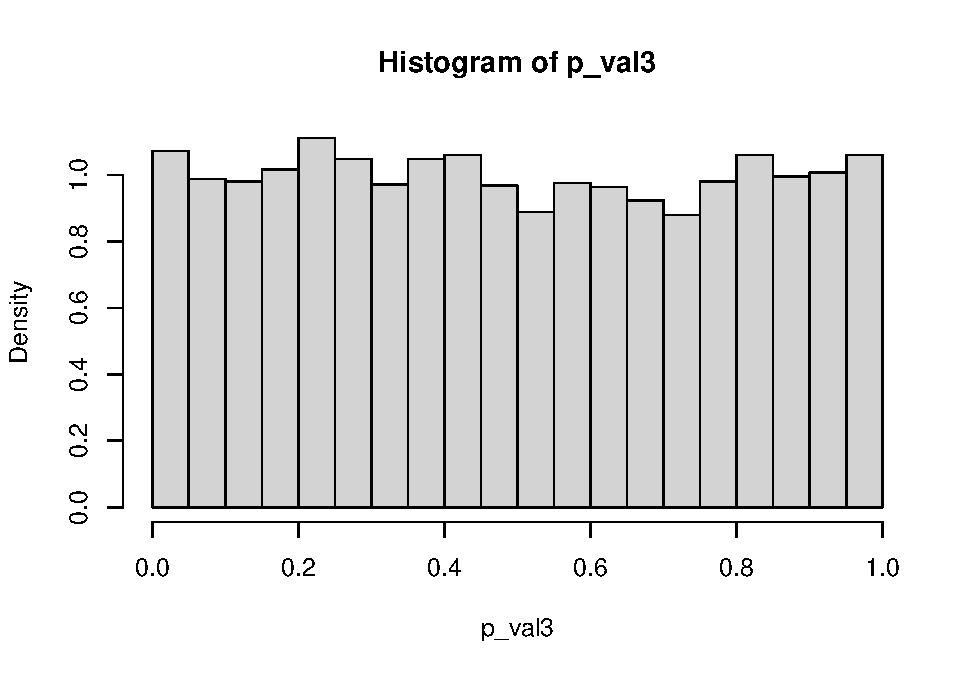
\includegraphics{stats-gene-research-progress-v4_files/figure-latex/unnamed-chunk-1-4.pdf}

\hypertarget{method-2}{%
\subsubsection{Method 2:}\label{method-2}}

This method takes much longer than the previous one, so we will not
aggregate the p-values as before. The approach will be illustrated
through two example: one without interaction and one with interaction:

\begin{Shaded}
\begin{Highlighting}[]
\KeywordTok{set.seed}\NormalTok{(}\DecValTok{123}\NormalTok{)}
\NormalTok{n =}\StringTok{ }\DecValTok{3000}
\NormalTok{p1 <-}\StringTok{ }\FloatTok{0.2}
\NormalTok{q1 <-}\StringTok{ }\DecValTok{1} \OperatorTok{-}\StringTok{ }\NormalTok{p1}
\NormalTok{beta0 <-}\StringTok{ }\FloatTok{-1.2}
\NormalTok{betaG <-}\StringTok{ }\FloatTok{0.8}
\NormalTok{betaE <-}\StringTok{ }\FloatTok{0.6}
\NormalTok{betaGE <-}\StringTok{ }\FloatTok{0.6}


\CommentTok{### Without interaction:}
\NormalTok{G =}\StringTok{ }\KeywordTok{apply}\NormalTok{(}\DataTypeTok{X =} \KeywordTok{rmultinom}\NormalTok{(n,}\DecValTok{1}\NormalTok{,}\DataTypeTok{prob =} \KeywordTok{c}\NormalTok{(p1}\OperatorTok{^}\DecValTok{2}\NormalTok{,}\DecValTok{2}\OperatorTok{*}\NormalTok{p1}\OperatorTok{*}\NormalTok{q1,q1}\OperatorTok{^}\DecValTok{2}\NormalTok{)) }\OperatorTok{>}\StringTok{ }\DecValTok{0}\NormalTok{, }\DataTypeTok{FUN =} \StringTok{"which"}\NormalTok{,}\DataTypeTok{MARGIN =} \DecValTok{2}\NormalTok{) }\OperatorTok{-}\StringTok{ }\DecValTok{1}
\NormalTok{E <-}\StringTok{ }\KeywordTok{rnorm}\NormalTok{(n, }\DataTypeTok{mean =} \DecValTok{0}\NormalTok{, }\DataTypeTok{sd =} \DecValTok{1}\NormalTok{)}
\NormalTok{latent_y <-}\StringTok{ }\NormalTok{beta0 }\OperatorTok{+}\StringTok{ }\NormalTok{betaG}\OperatorTok{*}\NormalTok{G }\OperatorTok{+}\StringTok{ }\NormalTok{betaE}\OperatorTok{*}\NormalTok{E  }\OperatorTok{+}\StringTok{ }\KeywordTok{rnorm}\NormalTok{(}\DataTypeTok{n =}\NormalTok{ n)}
\NormalTok{y <-}\StringTok{ }\KeywordTok{ifelse}\NormalTok{(latent_y }\OperatorTok{>}\StringTok{ }\DecValTok{0}\NormalTok{,}\DecValTok{1}\NormalTok{,}\DecValTok{0}\NormalTok{)}
\NormalTok{data <-}\StringTok{ }\KeywordTok{data.frame}\NormalTok{(}\DataTypeTok{y =}\NormalTok{ y, }\DataTypeTok{G =}\NormalTok{ G)}
\NormalTok{data}\OperatorTok{$}\NormalTok{OLRE <-}\StringTok{ }\DecValTok{1}\OperatorTok{:}\KeywordTok{nrow}\NormalTok{(data)}

\NormalTok{model11 <-}\StringTok{ }\KeywordTok{glmer}\NormalTok{(y}\OperatorTok{~}\StringTok{ }\NormalTok{G }\OperatorTok{+}\StringTok{ }\NormalTok{(}\OperatorTok{-}\DecValTok{1}\OperatorTok{+}\NormalTok{G}\OperatorTok{|}\NormalTok{OLRE), }\DataTypeTok{family =} \KeywordTok{binomial}\NormalTok{(}\DataTypeTok{link =} \StringTok{"probit"}\NormalTok{), }\DataTypeTok{data =}\NormalTok{ data, }\DataTypeTok{nAGQ =}\NormalTok{ 25L)}
\NormalTok{model12 <-}\StringTok{ }\KeywordTok{glm}\NormalTok{(y}\OperatorTok{~}\StringTok{ }\NormalTok{G,}\DataTypeTok{family =} \KeywordTok{binomial}\NormalTok{(}\DataTypeTok{link =} \StringTok{"probit"}\NormalTok{), }\DataTypeTok{data =}\NormalTok{ data)}
\KeywordTok{as.numeric}\NormalTok{((}\DecValTok{1} \OperatorTok{-}\StringTok{ }\KeywordTok{pchisq}\NormalTok{(}\DecValTok{2}\OperatorTok{*}\NormalTok{(}\KeywordTok{logLik}\NormalTok{(model11) }\OperatorTok{-}\StringTok{ }\KeywordTok{logLik}\NormalTok{(model12)), }\DataTypeTok{df =} \DecValTok{1}\NormalTok{))}\OperatorTok{/}\DecValTok{2}\NormalTok{)}
\end{Highlighting}
\end{Shaded}

\begin{verbatim}
## [1] 0.1817477
\end{verbatim}

\begin{Shaded}
\begin{Highlighting}[]
\CommentTok{### With interaction:}
\KeywordTok{set.seed}\NormalTok{(}\DecValTok{123}\NormalTok{)}
\NormalTok{latent_y <-}\StringTok{ }\NormalTok{beta0 }\OperatorTok{+}\StringTok{ }\NormalTok{betaG}\OperatorTok{*}\NormalTok{G }\OperatorTok{+}\StringTok{ }\NormalTok{betaE}\OperatorTok{*}\NormalTok{E }\OperatorTok{+}\StringTok{ }\NormalTok{betaGE}\OperatorTok{*}\NormalTok{G}\OperatorTok{*}\NormalTok{E }\OperatorTok{+}\StringTok{ }\KeywordTok{rnorm}\NormalTok{(}\DataTypeTok{n =}\NormalTok{ n)}
\NormalTok{y <-}\StringTok{ }\KeywordTok{ifelse}\NormalTok{(latent_y }\OperatorTok{>}\StringTok{ }\DecValTok{0}\NormalTok{,}\DecValTok{1}\NormalTok{,}\DecValTok{0}\NormalTok{)}
\NormalTok{data <-}\StringTok{ }\KeywordTok{data.frame}\NormalTok{(}\DataTypeTok{y =}\NormalTok{ y, }\DataTypeTok{G =}\NormalTok{ G)}
\NormalTok{data}\OperatorTok{$}\NormalTok{OLRE <-}\StringTok{ }\DecValTok{1}\OperatorTok{:}\KeywordTok{nrow}\NormalTok{(data)}
\NormalTok{model21 <-}\StringTok{ }\KeywordTok{glmer}\NormalTok{(y}\OperatorTok{~}\StringTok{ }\NormalTok{G }\OperatorTok{+}\StringTok{ }\NormalTok{(}\OperatorTok{-}\DecValTok{1}\OperatorTok{+}\NormalTok{G}\OperatorTok{|}\NormalTok{OLRE) ,}\DataTypeTok{family =} \KeywordTok{binomial}\NormalTok{(}\DataTypeTok{link =} \StringTok{"probit"}\NormalTok{), }\DataTypeTok{data =}\NormalTok{ data, }\DataTypeTok{nAGQ =}\NormalTok{ 25L)}
\NormalTok{model22 <-}\StringTok{ }\KeywordTok{glm}\NormalTok{(y}\OperatorTok{~}\StringTok{ }\NormalTok{G, }\DataTypeTok{family =} \KeywordTok{binomial}\NormalTok{(}\DataTypeTok{link =} \StringTok{"probit"}\NormalTok{), }\DataTypeTok{data =}\NormalTok{ data)}
\KeywordTok{as.numeric}\NormalTok{((}\DecValTok{1} \OperatorTok{-}\StringTok{ }\KeywordTok{pchisq}\NormalTok{(}\DecValTok{2}\OperatorTok{*}\NormalTok{(}\KeywordTok{logLik}\NormalTok{(model21) }\OperatorTok{-}\StringTok{ }\KeywordTok{logLik}\NormalTok{(model22)), }\DataTypeTok{df =} \DecValTok{1}\NormalTok{))}\OperatorTok{/}\DecValTok{2}\NormalTok{)}
\end{Highlighting}
\end{Shaded}

\begin{verbatim}
## [1] 1.201479e-06
\end{verbatim}

\end{document}
